\section{Introduction}

The blind source separation problem refers to the process of
recovering one or more signals that have been mixed in some unknown
manner and possibly also contamined by noise. Without any assumptions
on the mixing process, this problem is ill-poised. In practice
therefore, all BSS methods rely on some stylized fact about the nature
of the signals and/or the mixing process. It is therefore useful to
dichotomize BSS methods by these assumptions.


Arguably, two of the most important facts characterizing a mixing
process, are its temporal dynamics and the number of degrees of
freedom. The first point refers to whether the nature of the mixing
process changes over time, that is if the mixing matrix at time $t+k$
is different from that at time $t$ for $k>0$. The number of degrees of
freedom is the same concept as in linear algebra - the connection is
apparent by seeing the mixing process as a system of linear
equations. If $m$ is the number of observed signals and $n$ the number
of sources, the system is said to be \emph{underdetermined} if $m<n$
and conversely \emph{overdetermined} if $m>n$. 

\begin{figure}
  \centering
  \hrule
  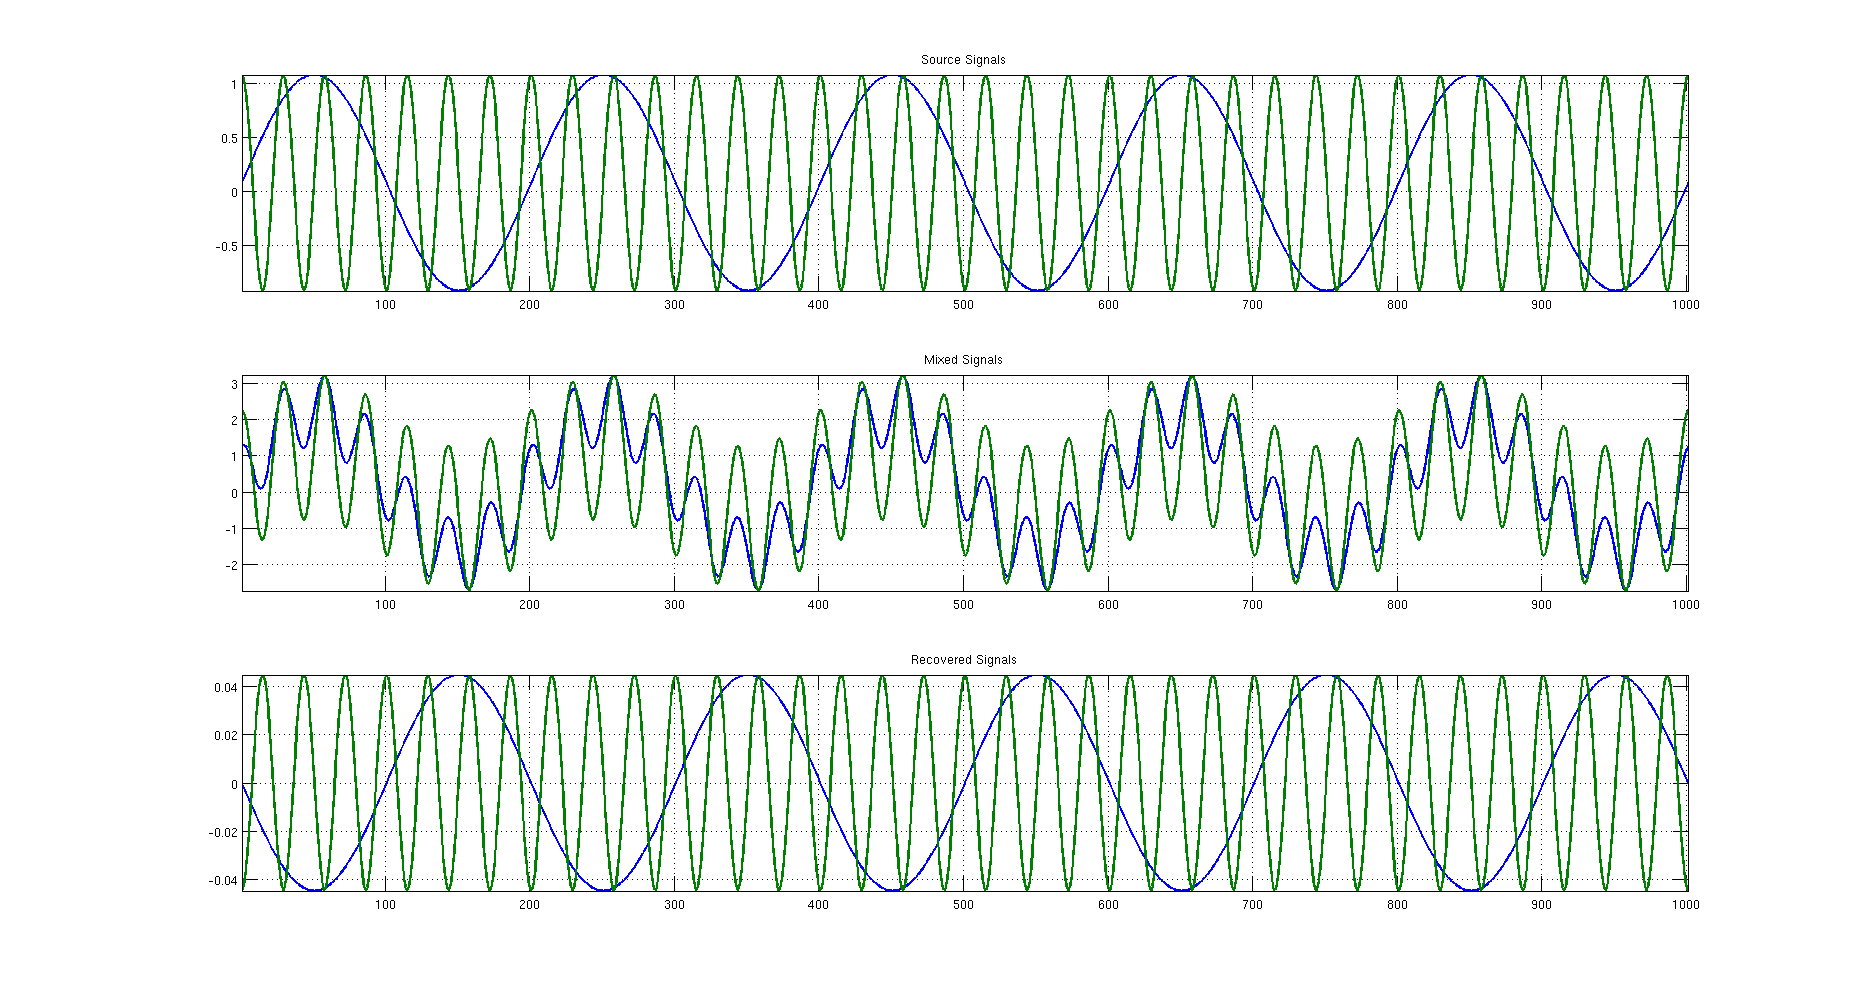
\includegraphics[width = .9\textwidth]{ica_simple}
  \hrule
  \caption{Stationary linear mixing process and separation.}
  \label{pca_time_series}
\end{figure}

We can also differentiate between method based on the nature of input
data. Early BSS research often considered the case of $n=m$, which
allows one to work with data in the time domain. For undetermined
systems, it is commonplace to work with some transformation of the
data, which in the case of audio data a time-frequency
representation. Common methods include the \emph{short-term Fourier
  transform} and the \emph{wavelet transform}.


The organization of this study is as follows. Section
\ref{reviewProcess} will briefly summarize the literature review
process, which is further documented by the underlying research
protocol given in Appendix \ref{protocol}. Section \ref{overview} is
a short description of the different techniques and methodologies found, summarised in section \ref{conclusion}.


\section{Literature Review Process}\label{reviewProcess} % Anders
The literature review process was conducted by manually searching searching the listed databases for published articles containing the predefined search terms.
The table below shows the amount of results presented to us when  using the more general of our search terms. Since the search terms we had defined gave us a large amount of results, we prioritized newer papers over older ones as per the Appendix \ref{protocol}.

\begin{table}[h]
\centering
	\begin{tabular}{|l|l|l|l|}
	\hline
	\textbf{Search term} & \textbf{CiteSeerX} & \textbf{Google Scholar} & \textbf{SpringerLink} \\
	\hline
	blind source separation & 292581 & 698000 & 13143\\
	blind audio source separation & 28612 & 26000 & 1072\\
	single channel blind source separation & 275543 & 78600 & 5024\\
	\hline
	\end{tabular}
\caption{Magnitude of hits on the most general terms}
\label{tab:myfirsttable}
\end{table}

After screening the results against the different criteria set in appendix \ref{protocol}, these papers were brought on for further consideration.

\begin{table} [ht]
    \begin{tabular}{|p{6cm}|p{4cm}|p{2cm}|}
        \hline
        \textbf{Title} & \textbf{Author} & \textbf{Published} \\ \hline
        Independent Component Analysis: a new concept? & Comon, P. & 1994\\ \hline
        An information maximization approach to blind separation and blind deconvolution  & Bell, A.J. and Sejnowski, T.J. & 1995\\ \hline
        A Context-Sensitive Generalization of ICA & Pearlmutter, B. A. and Parra, L. C. & 1996\\ \hline
        Independent Component Analysis & Hyvärinen, A. & 2001\\ \hline
        Blind One-Microphone Speech Separation: A Spectral Learning Approach & Bach, F.R. and Jordan, M.I. & 2004\\ \hline
        Fast and Robust Fixed-Point Algorithms for Independent Component Analysis & Hyvärinen, A. & 1999\\ \hline
        One Mincrophone Source Separation & Roweis, Sam T. & 2001\\ \hline
        Source separation using single channel ICA & Davies, M.E. and James, C.J. & 2007 \\ \hline
        Multidimensional Independent Component Analysis& Cardoso, J. L. & 1998\\ \hline
        Source Separation From Single-Channel Recordings by Combining Empirical-Mode Decomposition and Independent Component Analysis & Mijovic, B. De Vos, M., Gligorijevic, I., Taelman, J. and Van Huffel, S. & 2010\\ \hline
        Hidden Markov model decomposition of speech and noise & Varga, A. P., and R. K. Moore & 1990\\
        \hline
    \end{tabular}
\end{table}


\clearpage
\section{Literature Overview}\label{overview}



\subsection{Independent Component Analysis} %% Ulf

%% Standard ICA
Among the most common approaches to blind source separation is
independent component analysis (ICA). Common definitions of ICA use
either the maximization of independence or minimization of mutual information between the source
signals\footnote{It should be noted that while this text presents ICA
  in terms of blind source separation, the method is applicable to a
  wide array of machine learning problems including dimension
  reduction, classification, and de-noising.}. Formally, we can state
the ICA problem in terms of a generative model of the observed signals
$\mathbf{x}$, and the unknown a mixing matrix $\mathbf{W}$ and source
signals $\mathbf{s}$:


\begin{equation}
  \mathbf{x} =   \mathbf{W}  \mathbf{s}
\end{equation}

The AIM of the ICA process is to estimate the inverse mixing process
along with the original signals.

The classical reference on ICA
is \cite{comon94}, where the method of minimization of mutual
information between sources is presented. \cite{comon94} also presents an
analysis of the ambiguities and limitations of ICA, hereunder the permutation of
sources, scaling and non-gaussianity. 

There are several equivalent statements of ICA, which yields different
interpretations and computational models.
\cite{bellSejnowski95} proposes minimizing mutual information between
sources, as measured by \emph{differential entropy}. In this
implementation a feed-forward neural network structure is proposed.
Other approaches include conventional maximum likelihood (\cite{pearlmutterParra}) and maximization of
non-gausianity as measured by excess kurtosis. A popular approach is
the  FastICA algorithm (\cite{fastICA}) that minimizes mutual
information expressed by \emph{negentropy} by a fixed point method. 

The classic studies on ICA focus to a large extent on developing the
formal framework for ICA, and examples are largely centered on time
domain analysis in systems of an equal number of sensors and
sources\footnote{For a much more thorough survey on the classical literature 
on ICA, see \cite{hyvarinen2001}.}. ICA has however been extended to underdetermined systems and
the extreme case of single sensor systems. 

Many of these extensions are to a lesser extent changes to the
previously known algorithms; rather they involve transforming
the observed signals from the time domain to some other basis, the
most common of which are the frequency domain (Fourier transform), the
time-frequency domain (short-term Fourier transform) and the wavelet
domain. Compared to the time domain, the two latter are redundant
representations, but they transform the data so as to be suited for
ICA. \cite{mijovic2010} surveys variations on ICA as applied to single
channel recordings, hereunder single channel ICA (SCICA) and wavelet
ICA (WICA), in addition to proposing an algorithm that combines ICA
with empirical mode decompostion (EMD). EMD decomposes a signal into
independent components in the spectral domain and can be viewed as
similar to STFT.

The abovementioned approaches represent a select set of common
approaches to the  BSS problem. Other approaches rely to a larger
extent on direct application of knowledge about the human auditory
system. As an example \cite{bach} focuses on the problem on single channel speech
separation in the spectral domain by means of feature
maps where the features roughly corresponds to ``audible'' features such
as common onset, pitch, timbre and so forth. 

\newpage
\subsection{Hidden Markov Model Decomposition of Speech and Noise}
One of the earlier examples of using hidden Markov models for speech separation, are presented by A.P. Varga and R.K. Moore \cite{VargaHMMDecomp}. 
The approach described in this paper attempts to obtain the best estimate likelihood of an input observation conditioned on a particular state of the model and given the knowledge available about the contaminating noise. This is achieved with the use of parallel hidden Markov models, one for each of the components in the mixture signal to be decomposed. Given a two-component signal, the output generated from the model can be modelled as:

\begin{equation}\label{vargasEqn1}
Observational Probability = P(Observation|Hmm_1 \otimes Hmm_2)
\end{equation}

Recognition is carried out by extending the normal Viterbi equation to include the components desired to be decomposed:
\newline
\begin{equation}\label{vargasEqn2}
P_t(i,j) = \max_{u,v} P_{t-1} (u, v) a1_{u,i} a2_{v,j} b1_i \otimes b2_j (O_t)  \footnotemark
\end{equation}


By using this form of the Viterbi algorithm, this framework is able to simultaneously recognise different components of a mixture. It should be noted that this approach may be computationally difficult as the state search space grows in dimension for each component added.
Utilizing the fact that components rarely overlap in a certain frequency band, evaluation of the observation probability is approximated by:

\begin{equation}\label{vargasEqn3}
\begin{array}{lcl}
b1_i \otimes b2_j(O_t) &=&  P(max(O1_t, O2_t|i,j)) \\
\\ &  = &  C(O1_t,\mu1_i,\sigma1^2_i)N(O2_t, \mu2_j,\sigma2^2_j) + C(O2_t,\mu2_i,\sigma2^2_i)N(O1_t, \mu1_j,\sigma1^2_j)\footnotemark\\
\end{array}
\end{equation}


Initialization of the system consisted of supervised training on components, here being spoken numbers and noise. Utilizing a previously published algorithm for connected word recognition, the system was able to correctly classify speech contaminated with noise in the range -21 to + 15 dB. 
\footnotetext{$P_t(i, j)$ is the probability at time $t$ of the first component being in state $i$ and the second component in state $j$. $a1_{u,i}$ is the tranitional probability for the first component, likewise $a2_{v,j}$ is the transitional probability for the second component. $b1_i \otimes b2_j (O_t)$ is the observation probability}
\footnotetext{$C(O_t, \mu, \sigma)$ is the cumulative probability of all observation levels less than $O_t$ coming from a Normal distribution with mean $\mu$ and variance $\sigma^2$. Similarly $N(O_t, \mu, \sigma^2)$ is the probability of observation $O_t$ coming from a Normal distribution with mean $\mu$ and variance $\sigma^2$.}

\newpage
\subsection{Factoral Hidden Markov Models} %% Anders
The Hidden Markov modelling has been around since the late 1960s. Roweis\cite{roweisOneMic} proposes a technique called refiltering, where the idea is to separate sources in a mixed or corrupted recording. This is achieved through non stationary masking of the different frequency sub-bands from the target recording. Different sources may be isolated in the recording by changing the masking parameters. Using regularities in the spectrogram produced by a recording, it is possible to set the masking parameters, eg. common onset and offset. 

\begin{figure}[h]
  \centering
  \hrule
  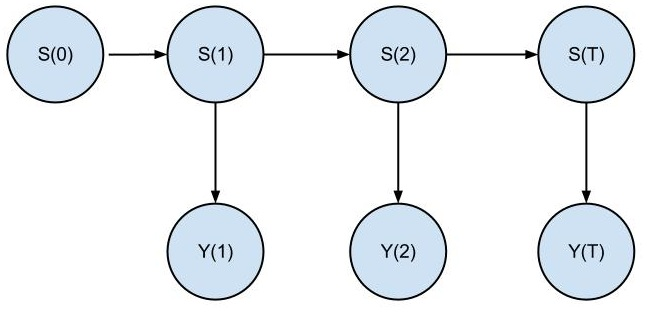
\includegraphics[width = .9\textwidth]{hmm}
  \hrule
  \caption{Hidden Markov Model}
  \label{hmm_figure}
\end{figure}



Training speaker dependent HMMs on isolated data from the sources to be separated, these models are then combined together in an architecture called factorial-max HMMs. The different HMMs evolve independently and for each observation vector produced at time t by each HMM, the elementwise maximum is chosen to create an observation. This is because the log magnitude spectrogram of a mixture of sources is very similar to the elementwise maximum of the individual spectrograms\footnote{This example was performed on two speakers. $a_{x_{t}}$ is the observation vector for speaker $x$ at time $t$, likewise is $b_{z_{t}}$ the observation vector for speaker $z$ at time $t$}. Separation is performed by setting the various masking signals to 1 or 0, depending on the observation vector at time $t$ for frequency band $i$.

\begin{figure}[h]
  \centering
  \hrule
  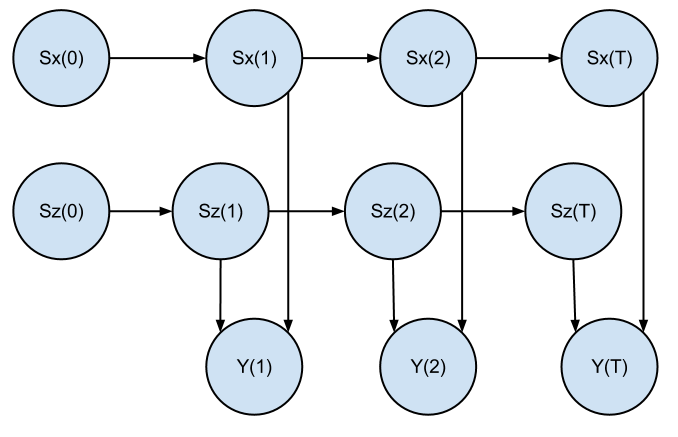
\includegraphics[width = .9\textwidth]{f_hmm}
  \hrule
  \caption{Factorial Hidden Markov Model}
  \label{fhmm_figure}
\end{figure}

The full generative model is given in Equations \ref{roweisEqn1} - \ref{roweisEqn3}.

\begin{equation}\label{roweisEqn1}
  p(x_{t}=j|x_{t-1}=i)=T_{ij}
\end{equation}

\begin{equation}\label{roweisEqn2}
  p(z_{t}=j|z_{t-1}=i)=U_{ij}  
\end{equation}

\begin{equation}\label{roweisEqn3}
  p(y_{t}|x_{t},z_{t})=N(max[a_{x_{t}},b_{z_{t}}], R)  
\end{equation}


\section{Conclusion}\label{conclusion}

In this survey we have provided an overview over some techniques in
blind source separation. Early work on blind source separation focused
to a large extent on time domain ICA. In extending the BSS problem to
multiple sources, the classical ICA method has been augmented by
adopting different signal representations, where the time-frequency
domain is particularly common. Different methods have also been
introduced, some borrowing from the human auditory system attempting
to hard-code domain specific knowledge. Others adopt different
algorithms; one important example here being hidden markov models
(HMMs). This is a very flexible approach to BSS as it allows for
non-stationary mixing, and relaxes many of the stringent assumptions
of classical ICA. 

\newpage
\appendix


\section{Research Agenda}\label{protocol}
The aim of this study is to systematically review current technology
for blind source separation (BSS), with particular emphasis on the
particular subproblem of single channel blind source separation
(SCBSS); that is, the recovery of several source signals from one observed signals.


\subsection{Background}
The blind source separation problem consists transforming a set of observed signals that has undergone some particular mixing process back to the original unobserved signals. The “blind” part of the problem refers to the fact that the nature of the mixing process is unknown. From original research on the blind source separation problem, focus has shifted from the case where with as many, or more recording channels than original sources, to the case of fewer channels than original sources. An important subproblem that we wish to focus on is where we have only one recording and attempt to recover multiple sources.

Our approach is two-fold: firstly we wish to look at studies about the performance of current single channel separation methods. Secondly, we wish to gain a broader overview over the state of research on BSS.

\subsection{Research Questions}
\begin{enumerate}
  \item What are the different variations on the blind source
    separation problem, in particular as pertains to audio data.
  \item Which methodologies and algorithms are applied to the
    different variations of the blind source separation problem as identified in Question 1.
  \item What are the theoretical properties of the techniques
    identified in Question 2, and  what assumptions do they make about the nature of the sources and the mixing process?
  \item What empirical evidence is there to document the performance
    of the techniques identified in Question 2 as applied to the
    problems identified in Question 1?
\end{enumerate}



\subsection{Search Strategy}
In reviewing the BSS literature we conduct a search of the below databases based on a set of keywords listed below. To filter the results we introduce a set of criteria to judge the relevance and quality of the results.

\subsubsection{Databases}

\begin{itemize}
 \item \href{www.springerlink.com}{SpringerLink}
 \item \href {www.citeseerx}{CiteSeerX}
 \item \href{scholar.google.com}{Google Scholar}
\end{itemize}

\subsubsection{List of Search Terms}

\emph{blind source separation, single channel blind source separation, single mixture blind source separation, hidden markov blind source, single microphone blind source separation, blind source separation review, blind source separation survey, pca blind source separation, ica blind source separation, principal component analysis blind source separation, independent component analysis blind source separation}.



\subsubsection{Inclusion and Quality Criteria}
We wish to study how various methods and/or approaches by which blind source problem is solved, which constraints are imposed by these methods, and how well a BSS system based on these ideas perform on real-life data. To filter out the most important studies to this end, we adopt the following criteria.

\begin{description}
	\item Inclusion Criteria
		\begin{enumerate}
			\item The main concern of the study is the BSS
                          problem.
			\item The algorithmic design decisions in the study must be justified.
			\item The study describes a reproducible algorithm/method.
			\item The study focuses on blind source separation of auditory signals.
		\end{enumerate}
	\item Quality Criteria
		\begin{enumerate}
			\item The study presents empirical results.
			\item More recent studies are preferred.
			\item The described test data set is
                          reproducible.
                        \item The study should present novel
                          theoretical approaches/methodologies OR
                          empirical results about previously known methods. 
			\item Literature reviews should discuss single channel blind source separation.
			\item The study should describe which other algorithms/methods the proposed solution can be compared with and the performance measure used in comparison.
		\end{enumerate}
\end{description}
